\documentclass[conference]{IEEEtran}

\usepackage{cite}
\usepackage[pdftex]{graphicx}
% declare the path(s) where your graphic files are
\graphicspath{{images/}}

% Packages that are sometimes useful
%\usepackage{amsmath,amssymb,amsfonts}
%\usepackage{algorithmic}
%\usepackage{float}
\usepackage{hyperref}
\hypersetup{
    colorlinks=true,
    linkcolor=blue,
    filecolor=magenta,      
    urlcolor=cyan,
    pdftitle={Reviving the Lost Art of Combinator Graph Reduction}
    }

\urlstyle{same}

\usepackage{amsmath}
\DeclareMathOperator{\strict}{strict}
\DeclareMathOperator{\lazy}{lazy}
\DeclareMathOperator{\lazyeta}{lazy_\eta}
\DeclareMathOperator{\linear}{linear}

\usepackage{listings}

\usepackage{svg}
\usepackage{placeins}


\ifCLASSOPTIONcompsoc
    \usepackage[caption=false, font=normalsize, labelfont=sf, textfont=sf]{subfig}
\else
\usepackage[caption=false, font=footnotesize]{subfig}
\fi

\usepackage{pgfplots}
\pgfplotsset{compat=1.17}

\begin{document}

\title{Reviving the Lost Art of \\Combinator Graph Reduction}

\author{\IEEEauthorblockN{Daan de Graaf}
    \IEEEauthorblockA{\textit{Master's student Computer Engineering} \\
        \textit{TU Delft / Eindhoven University of Technology}\\
        Eindhoven, Netherlands \\
        d.j.a.degraaf@student.tudelft.nl / d.j.a.d.graaf@student.tue.nl}
}

\maketitle

\begin{abstract}
    % Rules of thumb
    % - 1 sentence background
    Combinator Graph Reduction was once the dominant execution strategy for lazy functional languages, but inefficient translation algorithms and lack of an open-source implementation caused the technique to fall into obscurity in the late 1980s.
    The traditional translation algorithm produces a combinator expression that is in the worse case quadratic in the size of the input.
    % - 1 sentence motive/problem
    Recently, Kiselyov proposed a new family of translation algorithms that generate smaller combinator expressions, with some variants being linear in the size of the input.
    While the effect on code size is known, the difference in runtime performance has remained unquantified.
    % - 1 sentence objective
    Our goal is to find out how the reduction in code size affects execution time on a modern, efficient Combinator Graph Reduction engine.
    % - 1 sentence approach/method
    In absence of a suitable engine, we have developed our own based on the design of Miranda and TIGRE.
    We compile a set of test programs with Kiselyov's translation algorithms and measure their execution time on our best engine.
    % - 2 sentences support

    Our benchmarks show that our Miranda-style engine outperforms the original Miranda, and is therefore a good reference point to measure performance improvements against.
    We find that the threaded code approach proposed in TIGRE reduces the number of instructions and data accesses needed to execute programs, but frequent cache misses make it unattractive on architectures with split instruction and data caches.
    Kiselyov's new translation algorithms are shown to significantly boost performance in our benchmarks.
    The effect on execution time is even greater than we observe on code size.
    % - 1 sentence conclusion
    We conclude that the new translation algorithms significantly improve performance, and there may be further gains to be had by combining ideas from the different translation algorithms.

    %Many opportunities remain to improve the basic combinator graph reduction engine, such as the integration of other ideas from TIGRE, a concurrent garbage collector, and parallel reduction.
    % - 1 sentence implication
    %Our results show that there are significant improvements to be made in this area of research that has been largely static in recent years, and we hope there will be renewed interest from the community to do research in this field.
\end{abstract}

\begin{IEEEkeywords}
    combinatory logic, graph reduction, lazy functional language, lazy evaluation
\end{IEEEkeywords}

\section{Submission}
Submitted in partial fulfillment of the requirements for completion of the TU Eindhoven course Advanced Functional Programming (Capita Selecta SET, 2IMP05), under the guidance of prof. Tom Verhoeff.

\section{Introduction}
% Why did I research this? Give the motive, usually a knowledge gap or problem
Lazy evaluation of programs is a powerful idea.
It allows a program to operate on infinitely large data structures, and if part of the computation turns out to be unnecessary, it is more efficient than a strict evaluation.
In practice, delaying computation often introduces overhead, making languages based on lazy evaluation slower than their strict counterparts.
To compete with a strict implementation, a lazy runtime must maximize laziness while minimizing overhead.
It is a difficult balance, and over the years many different evaluator designs, or \textit{abstract machines}, have been proposed~\cite{turner_new_1979,kieburtz_g-machine_1985,fairbairn_tim_1987,burn_spineless_1988,koopman_fresh_1989,jones_implementing_nodate}.

One of the early approaches to implementing lazy functional languages is combinator graph reduction~\cite{turner_new_1979}.
It was the basis for David Turner's Miranda language~\cite{turner_miranda_1985}, the popular choice for pure functional languages and one of the few to be commercially supported at the time.
Eventually, the interest in Miranda and combinator graph reduction with it waned.
Part of the reason may be that Miranda was until very recently closed-source, licensed software (its source code was released only in 2020~\cite{turner_open_2021}), leading to the creation of the open-source Haskell language~\cite{hudak_history_2007}.
But combinator reduction also deserves part of the blame.
% Firstly, owing to the simplicity of individual combinators, expressions are reduced in many small steps, so the per-step overhead greatly impacts runtime performance.
% Every reduction step modifies the stack and usually also the graph, resulting in high memory traffic.
One of the major issues is that the translation to combinators may result in much larger programs.
For a lambda calculus expression of size $N$, the traditional bracket abstraction algorithm produces an output of $O(N^2)$ in the worst case, where other approaches such as supercombinators are linear\cite{spj_impl}.
Along with other disadvantages, this led to combinator graph reduction being all but abandoned.

% What did I research?
% - Research problem/question
%   * Definitions
%   * Choices
%   * Presuppositions
% - Why specifically this research question?
%   * Theoretical or societal relevance
Recently, however, a new algorithm for the translation of lambda calculus expressions into combinatory logic has been proposed that is linear in the size of the input\cite{kiselyov_lambda_2018}.
Kiselyov's translation algorithm is based on semantics rather than syntax and this deeper understanding of the program has been shown to produce more compact translations.
While a clear improvement over previous translation strategies, it remains to be seen how big the impact is on real-world performance.
Is it enough to bridge the performance gap with newer reduction engines based on different paradigms?
This leads us to our first research question:

\textbf{RQ1:} Does Kiselyov's semantic translation make combinator graph reduction competitive with contemporary lazy functional evaluators?

% How did I research this?
% - Methods
% - Sub-questions
We compare Kiselyov's translation algorithm to bracket abstraction by compiling a set of benchmark programs and measuring their execution time.
Future work will add GHC as a reference point for a contemporary evaluator, along with additional benchmark programs.

We also need a fast Combinator Graph Reduction engine that can run programs compiled to combinator expressions.
Alas, there is no performant reduction engine tailored to executing such programs.
The now open-sourced Miranda software is a good starting point, but it is showing its age.
The 2020 port compiles cleanly on a recent GCC, but enabling optimizations is known to break the garbage collector (Section~\ref{sec:miranda} covers this issue in more detail).
Miranda's architecture is based on cells with a tag, head, and tail as described in\cite{turner_new_1979}, but later work has shown that a tagless representation with direct pointers to code leads to better performance\cite{koopman_fresh_1989}.
In absence of an up-to-date reference on building a practical combinator reduction engine, we formulate the second research question:

\textbf{RQ2:} How is combinator graph reduction implemented efficiently on general-purpose hardware?

We evaluate the state of the art in combinator graph reduction and build a fast implementation for a language that is simple but powerful enough to express our benchmark programs.
Using this engine, we can then answer \textbf{RQ1}.

% How did I organize the report?
% - Structure Overview
Concretely, our contributions are the following:
\begin{itemize}
    \item Kiselyov develops not one but two algorithms. The first does not have linear complexity but tends to produce very compact code.
          The second is guaranteed to be of linear complexity, at the cost of being less compact in certain cases.
          Kiselyov's description requires that the reader be familiar with OCaml and the tagless-final style of programming.
          In Section~\ref{sec:kiselyov} we describe both algorithms in a more conventional style that is directly implementable in a general-purpose language.
    \item We implement a fast combinator graph reduction engine based on the ideas in Miranda~\cite{turner_miranda_1985} and later improvements~\cite{koopman_architecture_1992}.
          We elaborate on its design in Sections~\ref{sec:miranda} and~\ref{sec:tigre}.
    \item We evaluate the performance of Miranda, our engines, and Kiselyov's translation algorithms on a set of benchmark programs in Section~\ref{sec:eval}.
\end{itemize}

For readers unfamiliar with lambda calculus, combinatory logic or bracket abstraction, we provide a short introduction to these topics in Section~\ref{sec:prelim}.

\section{Preliminaries}
\label{sec:prelim}
\textbf{TODO: write section. Currently contains only a few small fragments}
\subsection{Lambda Calculus}

\subsection{Combinatory Logic}
Starting from a lambda calculus expression, we first translate it into an expression consisting exclusively of the application of a small set of predefined functions, or \textit{combinators}.
It turns out that any lambda calculus expression can be expressed using just three combinators:
\begin{itemize}
    \item $S \ f \ g \ x = f \ x \ (g \ x)$
    \item $K \ x \ y = x$
    \item $I \ x = x$\footnote{It turns out that $SKK = I$, so even this combinator is not strictly necessary, but all reasonable implementations do include $I$, and it simplifies the example.}
\end{itemize}

For example, $\lambda x.x+1$ can be converted into the combinator expression:

\[
    S \ (S \  (K \  +) \  I) \ (K \ 1)
\]

We invite the reader to verify this by applying $x$ to this expression and reducing it to $x+1$ with the usual $\beta$-reduction rule.
While the generated expression is not as easy to read, the simplicity of its components is appealing: to execute a program compiled to combinators, an evaluator only needs to support four operations: the built-in $S$, $K$ and $I$ combinators, and function application\footnote{And any builtins of the language, like the plus operator in the example.}.
Better still, conversion to combinators removes all bound variables.
The runtime need not concern itself with passing arguments, this is all handled by the combinators.
The compiled program is executed using graph reduction, a technique that is also common in other reduction engines\cite{kieburtz_g-machine_1985,fairbairn_tim_1987}.

\subsection{Bracket Abstraction}

\subsection{Graph Reduction}
Must cover: outermost reduction.

\section{Kiselyov's algorithms}
\label{sec:kiselyov}
Kiselyov's paper~\cite{kiselyov_lambda_2018} describes three iterations of his non-linear semantic translation, and finally the linear algorithm.
They are presented as a type system accompanied by an operational semantics, except for the $\eta$-optimization, which is given as an OCaml code patch.
OCaml's type system can represent these algorithms very concisely in a tagless-final style.
Below we describe the same algorithms in a more conventional style.
Our description places no requirements on the type system and can be directly implemented in any general-purpose programming language.
For the first and most basic algorithm, we give full definitions of all functions inline.
Definitions for the more advanced algorithms are given in Appendix~\ref{app:kiselyov}.

\subsection{Strict algorithm}
This is based on the rules in Figure 6 of Kiselyov's paper.
We call it \textit{strict} it does not have lazy weakening: most notably it lacks the K-optimization required for full laziness.

The most naive implementation is to perform the type checking, then use the built context to apply the elimination rules and the translated program.
As Kiselyov already notes in his treatment of the linear algorithm further on in the paper, the translation does not actually care what elements are in the context, just that we keep track of the size of the context.
This lets us express compilation as a recursive function, shown in Figure~\ref{fig:strict}.

\begin{figure}
    \begin{equation*}
        \begin{array}{l l l l}
            \strict & z         & = & 1 \models I                                              \\
            \strict & s \ e     & = & n+1 \models (0 \models K) \coprod (n \models c)          \\
                    &           &   & \text{where } (n \models c) := \strict e                 \\
            \\
            \strict & \lambda e & = & 0 \models K \; c                                         \\
                    &           &   & \text{where } (0 \models c) := \strict e                 \\
            \strict & \lambda e & = & (n-1) \models K \; c                                     \\
                    &           &   & \text{where } (n \models c) := \strict e                 \\
            \\
            \strict & e_1 \ e_2 & = & (n \models ((n_1 \models c_1) \coprod (n_2 \models c_2)) \\
                    &           &   & \text{where } (n_1 \models c_1) := \strict e_1           \\
                    &           &   & \text{where } (n_2 \models c_2) := \strict e_2           \\
                    &           &   & \text{where } n := \max n_1 \, n_2                       \\
        \end{array}
    \end{equation*}
    \centering
    \caption{Compilation function for the $\strict$ algorithm.}
    \label{fig:strict}
\end{figure}

There are two cases for $\lambda e$, and this is precisely where the number of elements in the context matters:
if the context is empty, the first rule applies, otherwise, we use the second one.
The semantic function may be defined as in Figure~\ref{fig:strict-sem}.

\begin{figure}
    \begin{equation*}
        \arraycolsep=1.4pt
        \begin{array}{l l l l l}
            (0 \models c_1)   & \coprod & (0 \models c_2)   & = & c_1 \ c_2                                         \\
            \\
            (0 \models c_1)   & \coprod & (n_2 \models c_2) & = & (0 \models B c_1) \coprod (n_2 - 1 \models c_2)   \\
            \\
            (n_1 \models c_1) & \coprod & (0 \models c_2)   & = & (0 \models C C c_2) \coprod (n_1 - 1 \models c_1) \\
            \\
            (n_1 \models c_1) & \coprod & (n_2 \models c_2) & = & (n_1 - 1 \models (s \coprod l)) \coprod r)        \\
                              &         &                   &   & \text{where } s := (0 \models S )                 \\
                              &         &                   &   & \text{where } l := (n_1-1 \models c_1 )           \\
                              &         &                   &   & \text{where } r := (n_2-1 \models c_2 )           \\
        \end{array}
    \end{equation*}
    \centering
    \caption{Semantic function for the $\strict$ algorithm.}
    \label{fig:strict-sem}
\end{figure}

These simplified functions can be implemented directly and efficiently in a conventional programming language.

\subsection{Lazy weakening}
Adding lazy weakening requires that we track which items in the context are ignored.
We change our context representation from an integer to a list of boolean values.
In the new compilation functions below, we use a shorthand $t$ for the value \textit{true} and $f$ for \textit{false}.
We always match the last element of lists and represent the remainder of the list with $\Gamma$.

\begin{equation*}
    \begin{array}{l l l l}
        \lazy & z         & = & t \models I                                                             \\
        \lazy & s \ e     & = & \Gamma,f \models c                                                      \\
              &           &   & \text{where } (\Gamma \models c) := \lazy e                             \\
        \\
        \lazy & \lambda e & = & \emptyset \models K \; c                                                \\
              &           &   & \text{where } (\emptyset \models c) := \lazy e                          \\
        \lazy & \lambda e & = & (\emptyset \models K) \coprod (\Gamma \models c)                        \\
              &           &   & \text{where } (\Gamma,f \models c) := \lazy e                           \\
        \lazy & \lambda e & = & \Gamma \models K \; c                                                   \\
              &           &   & \text{where } (\Gamma,t \models c) := \lazy e                           \\
        \\
        \lazy & e_1 \ e_2 & = & (\Gamma \models ((\Gamma_1 \models c_1) \coprod (\Gamma_2 \models c_2)) \\
              &           &   & \text{where } (\Gamma_1 \models c_1) := \lazy e_1                       \\
              &           &   & \text{where } (\Gamma_2 \models c_2) := \lazy e_2                       \\
              &           &   & \text{where } \Gamma := \Gamma_1 \sqcup \Gamma_2                        \\
    \end{array}
\end{equation*}

We have introduced yet another case for $\lambda e$, this time to distinguish between $t$ or $f$ as the last element in the context of the inner expression.
There is also the new function $\sqcup$, which we need to implement:

\begin{equation*}
    \begin{array}{l l l l l}
        \Gamma_1    & \sqcup & \emptyset   & = & \Gamma_1                     \\
        \emptyset   & \sqcup & \Gamma_2    & = & \Gamma_2                     \\
        \Gamma_1,t  & \sqcup & \Gamma_2,\_ & = & (\Gamma_1 \sqcup \Gamma_2),t \\
        \Gamma_1,\_ & \sqcup & \Gamma_2,t  & = & (\Gamma_1 \sqcup \Gamma_2),t \\
        \Gamma_1,f  & \sqcup & \Gamma_2,f  & = & (\Gamma_1 \sqcup \Gamma_2),f \\
    \end{array}
\end{equation*}

In our implementation, we unroll the recursion into a while loop and repeatedly pop elements from the two arrays until both are empty.
This builds the new context back to front, so as a final step, the array is reversed.

Alternatively, an implementation can pad the shorter list (at the start!) with $f$ and zip them.
This is particularly convenient for languages that provide a zip function with a default value\footnote{such as \href{https://docs.python.org/3/library/itertools.html\#itertools.zip\_longest}{\texttt{ziplongest}} in Python.}.

Our semantic function now has to handle more cases, and thus is somewhat larger:

\begin{equation*}
    \arraycolsep=1.4pt
    \begin{array}{l l l l l}
        (\emptyset \models c_1)  & \coprod & (\emptyset \models c_2)  & = & c_1 \ c_2                                                \\
        \\
        (\emptyset \models c_1)  & \coprod & (\Gamma_2,t \models c_2) & = & (\emptyset \models B c_1) \coprod (\Gamma_2 \models c_2) \\
        \\
        (\Gamma_1,t \models c_1) & \coprod & (\emptyset \models c_2)  & = & (\emptyset \models C C c_2) \coprod (\Gamma \models c_1) \\
        \\
        (\Gamma_1,t \models c_1) & \coprod & (\Gamma_2,t \models c_2) & = & (\Gamma_1 \models (s \coprod l)) \coprod r)              \\
                                 &         &                          &   & \text{where } s := (\emptyset \models S )                \\
                                 &         &                          &   & \text{where } l := (\Gamma_1 \models c_1 )               \\
                                 &         &                          &   & \text{where } r := (\Gamma_2 \models c_2 )               \\
        \\
        % The new additions
        (\Gamma_1,f \models c_1) & \coprod & (\Gamma_2,f \models c_2) & = & (\Gamma_1 \models c_1) \coprod (\Gamma_2 \models c_2)    \\
        \\
        (\Gamma_1,f \models c_1) & \coprod & (\Gamma_2,t \models c_2) & = & (\Gamma_1 \models (b \coprod l)) \coprod r)              \\
                                 &         &                          &   & \text{where } b := (\emptyset \models B )                \\
                                 &         &                          &   & \text{where } l := (\Gamma_1 \models c_1 )               \\
                                 &         &                          &   & \text{where } r := (\Gamma_2 \models c_2 )               \\
        \\
        (\Gamma_1,t \models c_1) & \coprod & (\Gamma_2,f \models c_2) & = & (\Gamma_1 \models (c \coprod l)) \coprod r)              \\
                                 &         &                          &   & \text{where } c := (\emptyset \models C )                \\
                                 &         &                          &   & \text{where } l := (\Gamma_1 \models c_1 )               \\
                                 &         &                          &   & \text{where } r := (\Gamma_2 \models c_2 )               \\
        \\
        (\emptyset \models c_1)  & \coprod & (\Gamma_2,f \models c_2) & = & (\emptyset \models c_1) \coprod (\Gamma_2 \models c_2)   \\
        \\
        (\Gamma_1,f \models c_1) & \coprod & (\emptyset \models c_2)  & = & (\Gamma_1 \models c_1) \coprod (\emptyset \models c_2)   \\
    \end{array}
\end{equation*}

The first 4 cases are direct translations from the previous definitions, the others are new additions to handle ignored elements.
The last 2 cases are not included in the original paper, but they are necessary to make the pattern matching exhaustive, and are present in the reference OCaml implementation.

\subsection{Eta optimization}
Kiselyov covers eta optimization as a change to his OCaml code rather than typing rules.
Our recursive functions are derived from the typing rules, so these changes are not as straightforward to incorporate.
%Previously Kiselyov's representation consisted of elements $C$, $N$ and $W$, representing closed expressions, a used context element, and an ignored context element respectively.
The introduction of the $V$ element means that a context may now be associated with either a closed expression or the top variable (we reuse $V$ as a marker for this).
Our implementation uses a tagged union to define a type that can be either an expression or the top variable.
For the compilation function, we only need to change the definition of $\lazyeta \ z$ and add an extra case for $\lazyeta \ \lambda e$:

\begin{equation*}
    \begin{array}{l l l l}
        \lazyeta & z         & = & \emptyset \models V                                                          \\
        \lazyeta & s \ e     & = & \Gamma,f \models c                                                           \\
                 &           &   & \text{where } (\Gamma \models c) := \lazyeta e                               \\
        \\
        \lazyeta & \lambda e & = & \emptyset \models I                                                          \\
                 &           &   & \text{where } (\emptyset \models V) := \lazyeta e                            \\
        \lazyeta & \lambda e & = & \emptyset \models K \; c                                                     \\
                 &           &   & \text{where } (\emptyset \models c) := \lazyeta e                            \\
        \lazyeta & \lambda e & = & (\emptyset \models K) \coprod_\eta (\Gamma \models c)                        \\
                 &           &   & \text{where } (\Gamma,f \models c) := \lazyeta e                             \\
        \lazyeta & \lambda e & = & \Gamma \models K \; c                                                        \\
                 &           &   & \text{where } (\Gamma,t \models c) := \lazyeta e                             \\
        \\
        \lazyeta & e_1 \ e_2 & = & (\Gamma \models ((\Gamma_1 \models c_1) \coprod_\eta (\Gamma_2 \models c_2)) \\
                 &           &   & \text{where } (\Gamma_1 \models c_1) := \lazyeta e_1                         \\
                 &           &   & \text{where } (\Gamma_2 \models c_2) := \lazyeta e_2                         \\
                 &           &   & \text{where } \Gamma := \Gamma_1 \sqcup_\eta \Gamma_2                        \\
    \end{array}
\end{equation*}

Our context merge function $\sqcup$ now also depends on the compiled expression, since we have a special case for $V$:

\begin{equation*}
    \begin{array}{l l l l l}
        (\Gamma_1,\_ \models c_1) & \sqcup_\eta & (\emptyset \models V)     & = & \Gamma_1,t                        \\
        (\emptyset \models V)     & \sqcup_\eta & (\Gamma_2,\_ \models c_2) & = & \Gamma_2,t                        \\
        (\emptyset \models c_1)   & \sqcup_\eta & (\emptyset \models V)     & = & t                                 \\
        (\emptyset \models V)     & \sqcup_\eta & (\emptyset \models c_2)   & = & t                                 \\
        (\emptyset \models V)     & \sqcup_\eta & (\emptyset \models V)     & = & \mathbf{impossible}               \\
        \\
        % Original ones
        (\Gamma_1 \models c_1)    & \sqcup_\eta & (\emptyset \models c_2)   & = & \Gamma_1                          \\
        (\emptyset \models c_1)   & \sqcup_\eta & (\Gamma_2 \models c_2)    & = & \Gamma_2                          \\
        (\Gamma_1,t \models c_1)  & \sqcup_\eta & (\Gamma_2,\_ \models c_2) & = & (\Gamma_1 \sqcup_\eta \Gamma_2),t \\
        (\Gamma_1,\_ \models c_1) & \sqcup_\eta & (\Gamma_2,t \models c_2)  & = & (\Gamma_1 \sqcup_\eta \Gamma_2),t \\
        (\Gamma_1,f \models c_1)  & \sqcup_\eta & (\Gamma_2,f \models c_2)  & = & (\Gamma_1 \sqcup_\eta \Gamma_2),f \\
    \end{array}
\end{equation*}

The $V$ value effectively encodes an additional implicit used element in the context.
We also have some new cases for the semantic function:

\begin{equation*}
    \arraycolsep=1.4pt
    \begin{array}{l l l l l}
        % Added for eta optimization
        (\Gamma_1,f \models c_1) & \coprod_\eta & (\emptyset \models V)    & = & c_1                                                        \\
        (\emptyset \models V)    & \coprod_\eta & (\Gamma_2,f \models c_2) & = & (\emptyset \models CI) \coprod_\eta (\Gamma_2 \models c_2) \\

        (\Gamma_1,t \models c_1) & \coprod_\eta & (\emptyset \models V)    & = & (\Gamma_1 \models (s \coprod_\eta l)) \coprod_\eta i       \\
                                 &              &                          &   & \text{where } l := (\Gamma_1 \models c_1 )                 \\
                                 &              &                          &   & \text{where } s := (\emptyset \models S )                  \\
                                 &              &                          &   & \text{where } i := (\emptyset \models I )                  \\
        (\emptyset \models V)    & \coprod_\eta & (\Gamma_2,t \models c_2) & = & (\emptyset \models SI) \coprod_\eta (\Gamma_2 \models c_2) \\
        (\emptyset \models c_1)  & \coprod_\eta & (\emptyset \models V)    & = & c_1                                                        \\
        (\emptyset \models V)    & \coprod_\eta & (\emptyset \models c_2)  & = & CI c_2                                                     \\
        (\emptyset \models V)    & \coprod_\eta & (\emptyset \models V)    & = & \mathbf{impossible}                                        \\
        \\

        (\Gamma_1 \models c_1)   & \coprod_\eta & (\Gamma_2 \models)       & = & (\Gamma_1 \models c_1) \coprod (\Gamma_2 \models)          \\
    \end{array}
\end{equation*}

The case $(\emptyset \models V) \coprod (\emptyset \models V) $ is impossible in this translation, implementations may throw an error or leave it as undefined behavior.
\textbf{TODO:} Why is this an impossible case?

With the addition of the expression value to $\sqcup_\eta$, the function now takes the same input as $\coprod_\eta$ and has very similar matching patterns.
Our implementation, therefore, folds context merging into $\coprod_\eta$ to make the code more concise.

\subsection{Linear algorithm}
The implementation of the linear algorithm is much simpler because it is based on the $\strict$ algorithm.
The compilation function is identical save for a different semantic function $\coprod_{\text{linear}}$:

\begin{equation*}
    \begin{array}{l l l l}
        \linear & z         & = & 1 \models I                                                              \\
        \linear & s \ e     & = & n+1 \models (0 \models K) \coprod (n \models c)                          \\
                &           &   & \text{where } (n \models c) := \linear e                                 \\
        \\
        \linear & \lambda e & = & 0 \models K \; c                                                         \\
                &           &   & \text{where } (0 \models c) := \linear e                                 \\
        \linear & \lambda e & = & (n-1) \models K \; c                                                     \\
                &           &   & \text{where } (n \models c) := \linear e                                 \\
        \\
        \linear & e_1 \ e_2 & = & (n \models ((n_1 \models c_1) \coprod_{\text{linear}} (n_2 \models c_2)) \\
                &           &   & \text{where } (n_1 \models c_1) := \linear e_1                           \\
                &           &   & \text{where } (n_2 \models c_2) := \linear e_2                           \\
                &           &   & \text{where } n := \max n_1 \, n_2                                       \\
    \end{array}
\end{equation*}

below we give the corresponding semantic function, which is no longer recursive, making this algorithm linear:

\begin{equation*}
    \arraycolsep=1.4pt
    \begin{array}{l l l l l}
        (0 \models c_1)   & \coprod & (0 \models c_2)   & = & c_1 \ c_2                               \\
        \\
        (0 \models c_1)   & \coprod & (n \models c_2)   & = & B_n \ c_1 \ c_2                         \\
        \\
        (n \models c_1)   & \coprod & (0 \models c_2)   & = & C_n \ c_1 \ c_2                         \\
        \\
        (n \models c_1)   & \coprod & (n \models c_2)   & = & S_n \ c_1 \ c_2                         \\
        \\
        (n_1 \models c_1) & \coprod & (n_2 \models c_2) & = & B_{n_2-n_1} \ (S_{n_1} \ c_1) \ c_2     \\
                          &         &                   &   & \text{where } n_1 < n_2                 \\
        (n_1 \models c_1) & \coprod & (n_2 \models c_2) & = & C_{n_1-n_2} \ (B_{n_1-n_2} \ c_1) \ c_2 \\
                          &         &                   &   & \text{where } n_1 > n_2                 \\
    \end{array}
\end{equation*}

\textbf{TODO: } Can we add lazy weakening and/or eta optimization?

\section{Miranda}
\label{sec:miranda}
For our base implementation of a Combinator Graph Reduction engine, we try to stick to Miranda's design as much as possible.
While there is published work on Miranda~\cite{turner_miranda_1985}, it does not provide much detail on the reduction engine.
Fortunately, the source code for Miranda is now freely available~\cite{turner_open_2021}, and from the code, we can deduce that its design is very similar to SASL~\cite{turner_new_1979}, an earlier language developed by Turner.

The approach we describe here is the one taken for our implementation, which may not fully correspond to Miranda's.
Not all implementation issues are fully described in the literature, and in places where Miranda's implementation was not clear to us either, we developed our own solution.
In particular, Section~\ref{sec:strict} covers \emph{our} approach to the resumption of the main reduction after arguments to strict combinators have been reduced, but this may be implemented differently in Miranda.

Miranda converts source programs into combinatory logic using Turner's modified bracket abstraction algorithm~\cite{turner_another_1979}.
The converted program, composed of combinators, constants and function application, is then loaded into a graph structure.
The graph is binary: every node has exactly two children, and the node itself represents the application of the left node to the right one.
Let us start with an example program $SKK \ 3$.
The $S$ combinator takes three arguments, but a node can only store the application to a single argument.
The left associativity of function application lets us rewrite the example program as $((SK) \; K)\ 3$.
In this form, it is straightforward to construct the associated binary graph, shown in Figure~\ref{fig:skk3}.

\begin{figure}
    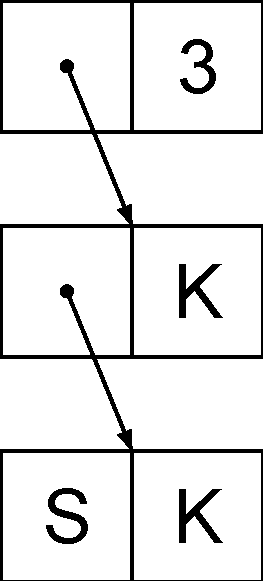
\includegraphics[width=.15\columnwidth]{skk3}
    \centering
    \caption{$SKK \ 3$ in graph representation.}
    \label{fig:skk3}
\end{figure}

To reduce this graph, we follow the left pointer until we find a combinator to apply.
As we traverse the graph along what is often called the \textit{spine}, we keep the nodes we have seen on a stack, because their right nodes contain the arguments to the combinator we eventually find.

In this example graph, after following two pointers we find the $S$ combinator, and we apply the definition $S f g x \Rightarrow (f x) (g x)$ to rewrite the graph, as shown in Figure~\ref{fig:skk3_sred}.

\begin{figure}
    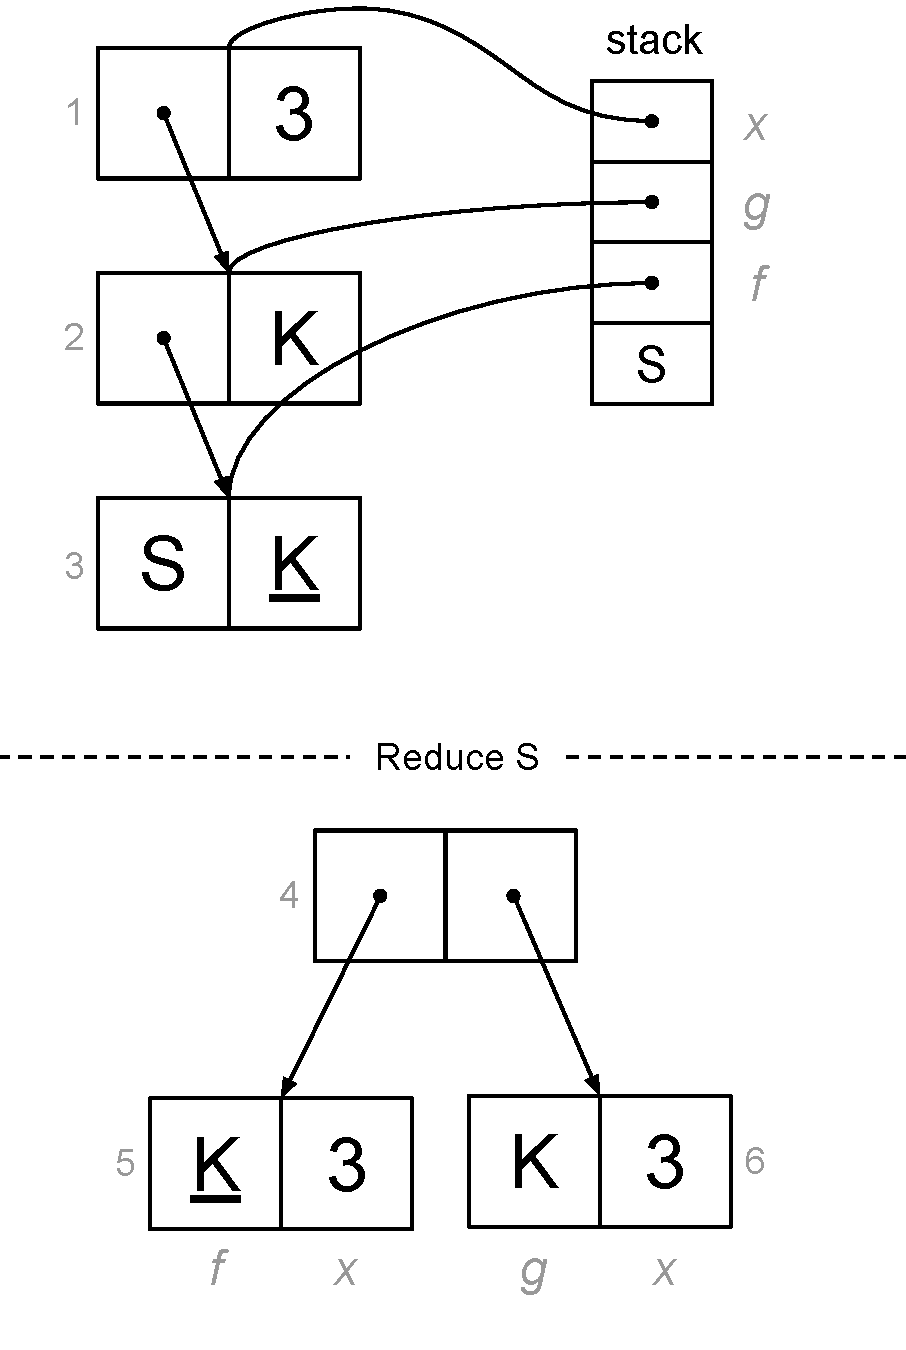
\includegraphics[width=.51\columnwidth]{skk3_sred}
    \centering
    \caption{
        First reduction step for $SKK \ 3$.
        One of the K combinators is underlined to make them easier to distinguish.
    }
    \label{fig:skk3_sred}
\end{figure}

The reduction process continues until the program has been reduced to a constant value, or there are insufficient arguments for the next combinator to reduce.
The expression is said to be in \textit{weak head normal form}: some inner part of the expression may be reducible, but we only perform outermost reduction, so this is as close as we can get to the normal form.

\subsection{Sharing}
In the reduction in Figure~\ref{fig:skk3_sred}, we have copied the value $3$ to two nodes.
For another reduction where the $x$ value is a pointer to a subgraph, performing the reduction may result in multiple pointers to the same expression.
Expressions in Miranda are \textit{referentially transparent}: we can safely replace any expression with the value it computes.
Computing $x$ in both branches would therefore be wasteful.
Instead, we would like to compute it once (in whatever branch runs first) and have the second branch directly reuse the result.
It turns out that this is not too difficult to implement: when we make a reduction step, we update the outermost node with the contents of the new outermost node.
In Figure~\ref{fig:skk3_sred}, this would mean we overwrite node 1 with the contents of node 4.
Now any other pointers to node 1 automatically point to the reduced equivalent.
If the expression reduces to a single value $v$ (say an integer), we can use the $I$ combinator to make an \textit{indirection node} $I v$.

\subsection{Representing the graph}
Miranda represents the graph using three arrays, \texttt{hd} (for head) stores the left pointer, \texttt{tl} (for tail) stores the right pointer, and \texttt{tag} stores metadata for the cell.
Owing to its early inception when 64-bit machines were rare, \texttt{hd} and \texttt{tl} are 32 bits wide.
\texttt{tag} only needs to store a few bit flags and thus is a single byte wide.
Our implementation stores two flags in \texttt{tag}:
\begin{itemize}
    \item \texttt{WANTED}: Set if this cell is currently in use. Cells without this bit set are considered free and may be overwritten to store new nodes in the graph. More on this in Section~\ref{sec:gc}.
    \item \texttt{RHS\_INT}: Set if the right pointer is not a pointer but an integer value. Note that the left pointer can never be an integer because the left pointer is always a function for which the right pointer is the first argument.
\end{itemize}

Miranda integers have unlimited precision, using GNU MP~\cite{gnump} internally.
For simplicity (and performance), our implementation instead treats the cell pointer as a 32-bit signed integer.

It is unclear why a representation with three separate arrays was chosen over a single array where each element contains a `cell' struct with a head, tail, and tag.
We suspect decomposing the graph into separate arrays leads to poor data locality, as almost any operation will access all three parts of a cell.
Our base implementation respects this design choice, later implementations do not.

Miranda reserves the lower range of cell pointer values for special purposes:
\begin{itemize}
    \item 0..255 represents the Latin 1 character set.
    \item 256..305 for internal use in the lexer.
    \item 306..446 to encode combinators.
\end{itemize}

The first 446 cells in the heap are unused: when the reduction engine encounters their value, they are interpreted as a character, lexer rule or combinator.
This explains why we have to tag integers but not combinators or character values.

Our implementation does not support character values and needs no reserved number for the lexer, so we can encode the first combinator as $0$.
The bulk combinators introduced by the $\linear$ algorithm do complicate the encoding somewhat:
in principle, there is now an infinite amount of possible combinators.
However, compiled programs only contain a finite subset of those combinators, and the reduction process only creates combinators that were present in the original program.
We can have an efficient encoding of combinators, but only if we generate it for specific programs.
Our implementation keeps an array of function pointers, each pointing to the code to reduce a particular combinator.
The array is populated as the compiled program is loaded into the graph representation:
when we encounter a combinator we have not seen before, its implementation is added to the array, and the combinator is encoded into the graph as its index into the array.
At runtime, combinator resolution is done by indexing into the array and calling the associated function.

\subsection{Strict combinators}
\label{sec:strict}
Miranda has special built-in combinators to perform arithmetic operations and compare numbers.
Where most combinators place no restrictions on their arguments, these combinators require their arguments to be fully reduced to integers (hence call them \textit{strict}), and so require special treatment.

When a \textit{strict} combinator is about to be reduced, the engine inspects the arguments.
If all arguments are reduced, the combinator reduction is performed as usual.
If one or more arguments are not yet reduced, we push the pointers to those arguments onto the stack and proceed to reduce from the top of the stack.
Eventually, the top argument will have been fully reduced, producing an integer value.
In general, if a reduction results in an integer value, it can mean one of two things:
\begin{itemize}
    \item The value is the result of the program.
    \item The value is one of the arguments for a strict combinator.
\end{itemize}
We distinguish between these cases by looking at the size of the stack: if it is empty, we have computed the final result of the program.
Otherwise, we continue reducing from the top of the stack, which will be either another argument or the original combinator expression.
The pointer to the original complex argument is replaced with an indirection node to the value, using the update logic described earlier.

As an example, consider the expression $+ \ 1 \ (K \ 2 \ 3)$.
After we have traversed the spine and encountered the $+$ combinator, the engine notices that the second argument is not yet reduced, and adds it to the stack.
Figure~\ref{fig:add_step1} shows the state of the graph at this point in the reduction process.

\begin{figure}
    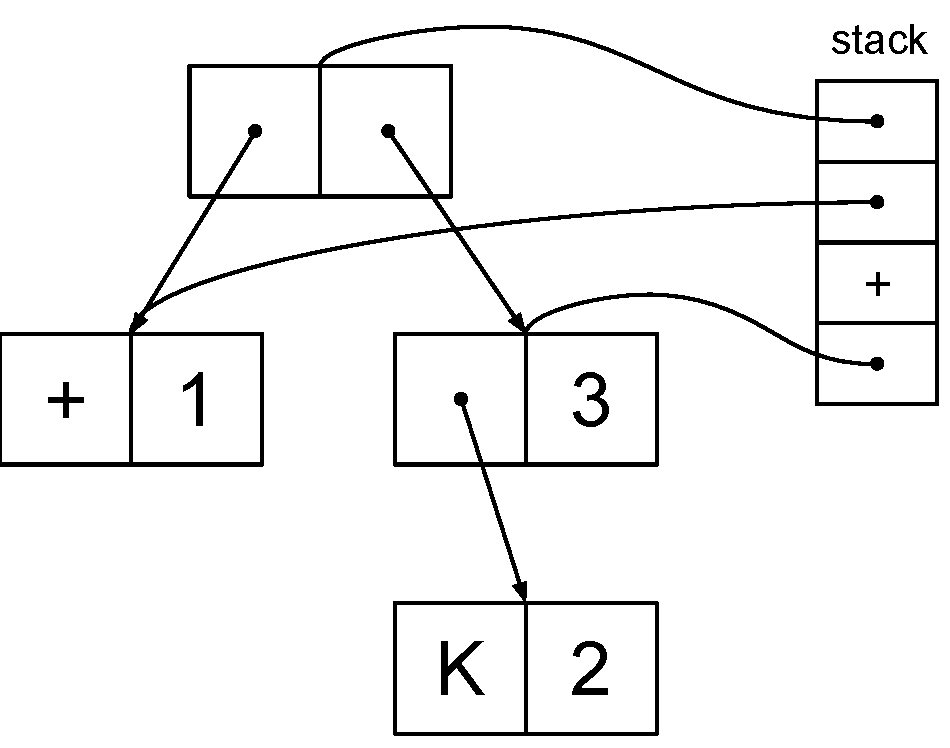
\includegraphics[width=.8\columnwidth]{add_step1}
    \centering
    \caption{
        Graph of $+ \ 1 \ (K \ 2 \ 3)$ after the second argument has been added to the stack.
    }
    \label{fig:add_step1}
\end{figure}

Once $K \ 2 \ 3$ has been reduced to $3$, the engine observes that the stack is not yet empty, so it creates an indirection node and resumes reduction from the top of the stack.
Figure~\ref{fig:add_step2} reflects this state.

\begin{figure}
    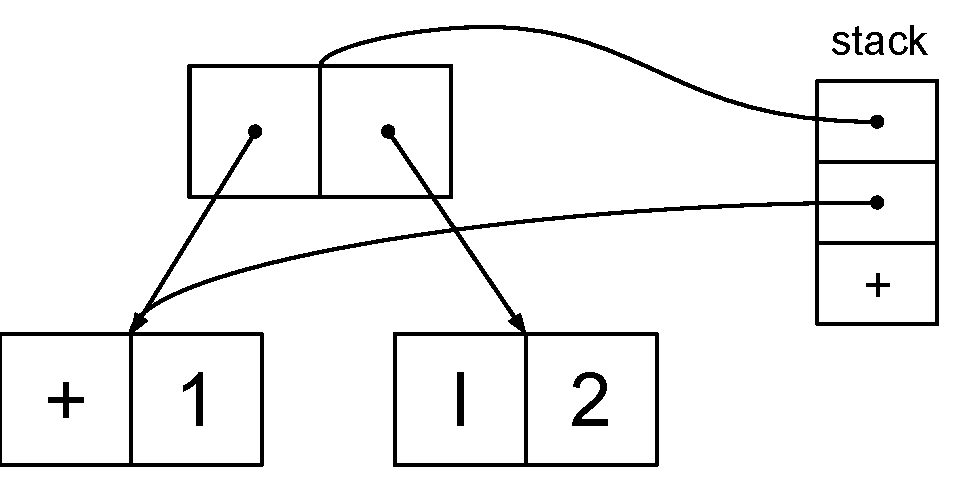
\includegraphics[width=.8\columnwidth]{add_step2}
    \centering
    \caption{
        Graph of $+ \ 1 \ (K \ 2 \ 3)$ after the second argument has been reduced.
    }
    \label{fig:add_step2}
\end{figure}

This example shows that it is not sufficient to check the \texttt{tag} of each argument to see if it is an integer: indirection nodes also count as fully reduced.

\subsection{Garbage collection}
\label{sec:gc}
The graph reduction process may lead to some nodes becoming unreachable.
Coming back to the example in Figure~\ref{fig:skk3_sred}, after the reduction step nodes 2 and 3 are no longer used: they are \textit{garbage}.
In this example, it is easy to conclude which nodes are garbage, but in larger programs, there are often multiple references to the same node, so we cannot mark nodes as garbage during the reduction step.
Miranda employs a simple mark-and-sweep garbage collector that kicks in when the engine runs out of free cells while allocating a new node.
In the first phase, it zeroes out the \texttt{WANTED} bit on all tags in the heap.
Then in the marking phase, starting from the elements currently on the stack\footnote{
    Miranda keeps its reduction stack on the C stack.
    This makes it difficult to reliably enumerate all cell pointers on the stack at a given point in time, because the compiler may choose to keep some of the pointers in registers.
    For this reason, users are instructed not to enable optimizations when compiling Miranda, which hurts performance but is necessary for correctness.
    When Miranda was developed, compilers were not advanced enough to perform such optimizations, so this was not an issue.
}, the garbage collector traverses the graph and sets the \texttt{WANTED} bit on all reachable nodes.
There is no real sweep phase: instead, the allocation routine walks over the tag array until it finds a cell that is not marked as \texttt{WANTED}.
This also means that there is no list of currently free cells, which we suspect may lead to performance issues in large heaps.

We consider the garbage collector in Miranda to be somewhat simplistic and inefficient, and we suspect there is much to improve in terms of efficiency.
Our benchmark programs do not use too much heap space, so we choose not to focus our efforts on this, and defer optimizations on this front to future work.

\section{TIGRE}
\label{sec:tigre}
The TIGRE engine, first presented in~\cite{koopman_fresh_1989}, is a combinator graph reduction engine like Miranda.
Originally designed for the VAX instruction set, our implementation targets the x86-64 instruction set but mirrors the TIGRE design otherwise.
The TIGRE paper focuses on key differences from Miranda, the elimination of tags and directly executable graph nodes, so where the paper omits implementation details we take the same approach as our reference implementation based on Miranda.

\subsection{Eliminating tags}
The TIGRE authors point to tags as a major source of inefficiency in graph reduction engines.
At evaluation time Miranda must check the tag of nodes to see if their right-hand side is a value or a pointer to a node.
TIGRE does away with this by adding a special \texttt{LIT} combinator.
The \texttt{LIT} combinator takes one argument guaranteed to be a literal value and returns it, like an \texttt{I} combinator specialized for constants.
An apparent downside of this is that simple expressions require more indirection, and therefore a larger graph to reduce.
Take for example the expression $1+2$, which in the Miranda-style engine can be represented with just two nodes, shown in Figure~\ref{fig:1_plus_2_miranda}.

\begin{figure}
    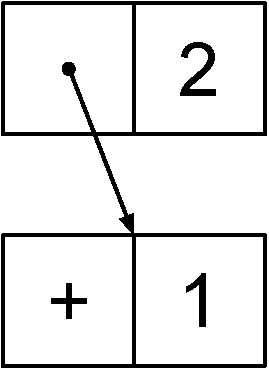
\includegraphics[width=.2\columnwidth]{1_plus_2_miranda}
    \centering
    \caption{
        Graph of $1 + 2$ in the Miranda-style engine.
        Tags omitted for brevity.
    }
    \label{fig:1_plus_2_miranda}
\end{figure}

The TIGRE version of this program, shown in Figure~\ref{fig:1_plus_2_tigre}, is larger, occupying four nodes.

\begin{figure}
    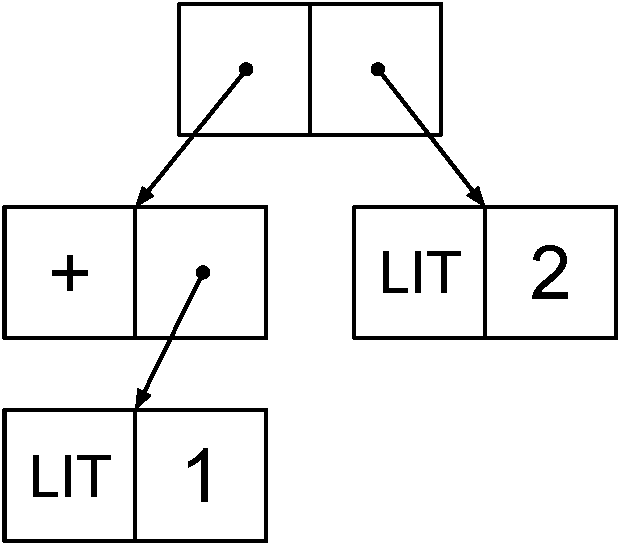
\includegraphics[width=.46\columnwidth]{1_plus_2_tigre}
    \centering
    \caption{
        Graph of $1 + 2$ in the TIGRE-style engine.
    }
    \label{fig:1_plus_2_tigre}
\end{figure}

In this example, the TIGRE graph may indeed be slower to evaluate, but the same does not hold for the programs in general.
If the values $1$ and $2$ were the results of a previous computation, they would also be behind an indirection node in the Miranda engine.
The TIGRE approach is only slower when performing operations on values that are constant in the source program, in other cases the reduced branching on tag values is expected to speed up execution.

The TIGRE authors report that some engines also use the tag to distinguish between combinators and cell pointers.
In Miranda the lowest cell pointers are reserved for combinators, so this does not need to be encoded in the tag, but the engine still needs to do a case distinction for low values of the pointer.
TIGRE also eliminates this overhead by encoding nodes as executable machine instructions.
We discuss this encoding in more detail in the next section.
With this change any pointer in the graph points to executable code: nodes are directly executable, and for combinators, we can insert a pointer to their implementation function.
The overhead of interpreting tags is thus fully eliminated.

Our implementation still has a tag byte in each cell, but it is exclusively used by the garbage collector to keep track of free and occupied cells.
The TIGRE paper provides no details on garbage collection, so we adopt the same mark-and-sweep collection approach as Miranda.

\subsection{Executable graph nodes}
Due to the elimination of tags, graph nodes must be executable x86-64 machine instructions.
Executing a node is expected to \emph{unwind the spine}: a pointer to the current node should be pushed onto the stack, after which we proceed to evaluate the cell to the left.
It turns out that this can be neatly encoded as a subroutine call in both the VAX and x86-64 instruction sets.

The x86-64 \texttt{CALL} \textit{rel32} instruction\footnote{\url{https://c9x.me/x86/html/file_module_x86_id_26.html}} modifies the processor state as follows:
\begin{enumerate}
    \item Pushes onto the stack a pointer to the instruction directly after the \texttt{CALL}.
          In a regular program, this is the \emph{return address}, the address the program should jump to after the subroutine finishes.
    \item Adds \textit{rel32} to the program counter register \texttt{\%rip}.
          \textit{rel32} encodes the address of the subroutine as a signed 32-bit offset from the location of the \texttt{CALL}.
\end{enumerate}

We exploit this by encoding nodes as a \texttt{CALL} instruction to the left pointer, followed by the right pointer as a raw value.
The memory layout of a node is illustrated in Figure~\ref{fig:tigre_layout}.

\begin{figure*}
    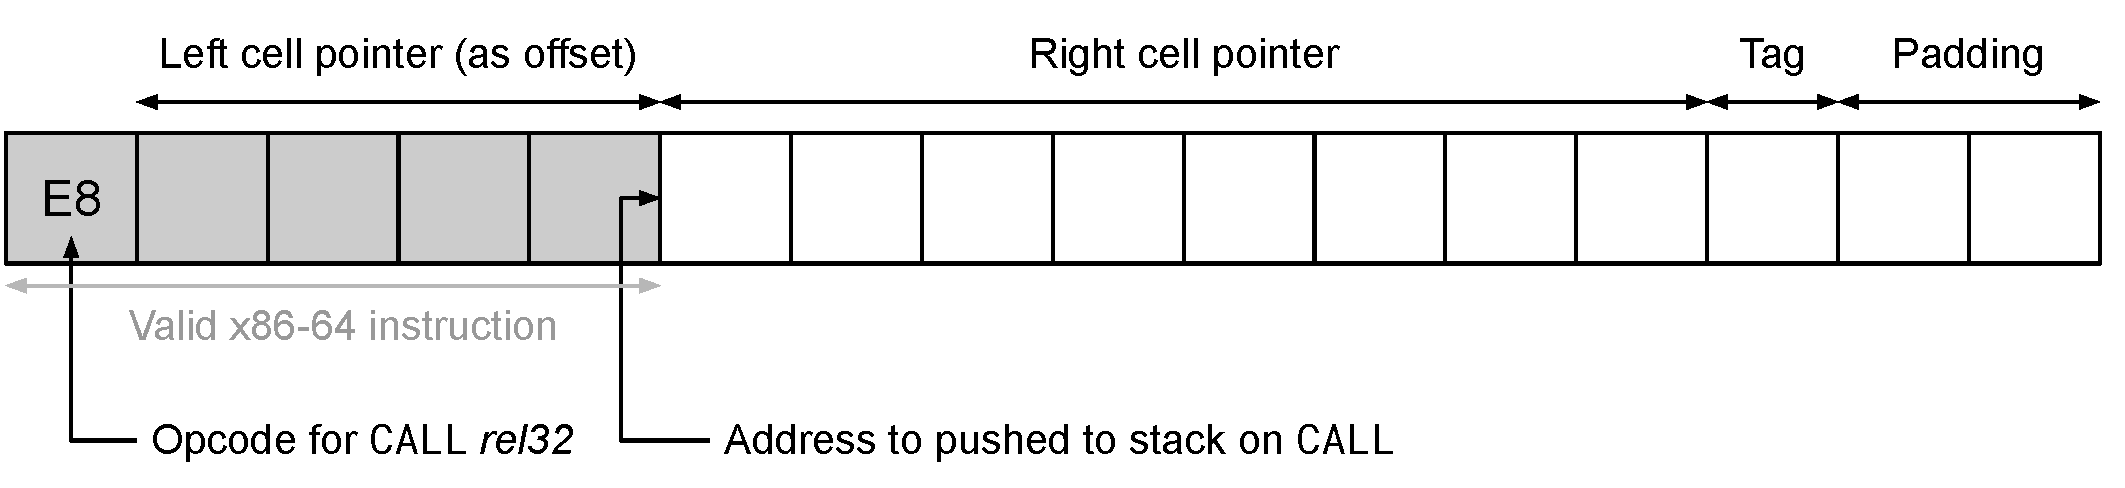
\includegraphics[width=2\columnwidth]{tigre_layout}
    \centering
    \caption{
        Memory layout of a node in the TIGRE-style engine.
        Each square represents a byte of memory.
    }
    \label{fig:tigre_layout}
\end{figure*}

When execution jumps to a node, the \texttt{CALL} instruction executes.
The address of the right pointer is pushed to the stack.
This is convenient because when later a combinator executes, it only needs to read the value of the right pointer (the left is only needed to unwind the stack).
Execution then jumps to the address of the left cell pointer, which is either another node or the code for a combinator.
The \texttt{CALL} instruction and 64-bit right pointer take up 13 bytes.
We add an extra byte to store the tag (only one bit is currently used) and 2 bytes of padding so the full node is 16 bytes wide.
Having 16-byte wide nodes is convenient because Intel processors can execute jumps faster if the target is aligned to a 16-byte boundary\footnote{\url{https://groups.google.com/g/golang-nuts/c/dhGbgC1pAmA/m/Rcqwcd5mGmoJ}}.

The simpler combinators are easily expressed as a short sequence of assembly instructions.
Figure~\ref{fig:combI} shows the implementation of the I combinator.

\begin{figure}
    \begin{lstlisting}[
        language={[x86masm]Assembler},
    ]
    comb_I:
        ; Pop pointer to argument
        ; into rax
        pop rax
        ; Dereference and jump
        jmp [rax]
    \end{lstlisting}
    \centering
    \caption{I combinator in x86-64 assembly.}
    \label{fig:combI}
\end{figure}

Combinators that return a value (\texttt{LIT} or strict combinators) can be implemented by computing the value and returning it with \texttt{RET}.
See for example the implementation of \texttt{LIT} in Figure~\ref{fig:combLIT}.

\begin{figure}
    \begin{lstlisting}[
        language={[x86masm]Assembler},
    ]
    comb_LIT:
        ; Pop pointer to argument
        ; into rax
        pop rax
        ; Dereference and store 
        ; in return value register
        mov rax, [rax]
        ; Return to caller
        ret
    \end{lstlisting}
    \centering
    \caption{LIT combinator in x86-64 assembly.}
    \label{fig:combLIT}
\end{figure}

A strict combinator that needs to evaluate its arguments is easier to implement in a TIGRE-style engine compared to Miranda: the implementation can strictly evaluate arguments by jumping to the argument node with a \texttt{CALL} instruction, and control will return to the combinator implementation after the argument has been evaluated and the \texttt{RET} instruction executes.
The fully evaluated argument is then available in the \texttt{\%rax} register.
This even works from Rust code: a pointer to a node can be cast to a function pointer with an integer as a return value and invoked normally.

\textbf{TODO: Maybe add a step-by-step reduction example?}

To our surprise, we did not find the TIGRE-style engine more difficult to implement than the Miranda version, mainly because the reduction process happens to map rather naturally to subroutine calls.
We discuss the main challenges encountered during the implementation in the next section.

\subsection{Implementation issues}
\subsubsection{Writeable and executable memory}
For our reduction engine to work, nodes must be stored in executable memory.
Modern x86-64 CPUs support the NX-bit~\cite{paulson_new_2004}, which allows the operating system to mark regions of the memory as non-executable, triggering an exception if a program jumps to a page with the NX-bit set.
The NX-bit is typically enabled by default on dynamically allocated heap memory.
To allocate memory without the NX-bit set on Linux, we allocate memory for the graph using \texttt{mmap}\footnote{\url{https://man7.org/linux/man-pages/man2/mmap.2.html}} with the \texttt{PROT\_EXEC} (to allow execution) and \texttt{PROT\_WRITE} (to allow writing) flags.
Some operating systems do not allow unprivileged programs to set \texttt{PROT\_EXEC} and \texttt{PROT\_WRITE} at the same time.
One solution to this is to flip the memory protection settings from executable to writeable, make the changes, and flip back to executable and continue execution~\cite{de_mooij_wx_2015}.
We anticipate this would be prohibitively expensive for our engine: After a combinator executes, it updates the graph with the new value, so that if the same value is used in a different subgraph, it is only evaluated once (just as Miranda does).
The engine would have to issue two \texttt{mprotect} system calls at every reduction step, a heavy performance penalty.
Luckily, the author's Linux distribution does not enforce a W \^{} X policy and allows the allocation of memory that is both writeable and executable.

\subsubsection{Relative jumps}
The \texttt{CALL} instruction takes as argument a 32-bit offset relative to the instruction pointer (the address of the \texttt{CALL} instruction), rather than a full 64-bit address.
Therefore, some pointer arithmetic is required to calculate the value of this offset.
More importantly, a 32-bit offset is too small to reach any target within the 64-bit address space.
This is problematic for large programs where nodes may be very far apart.
The programs we have used to evaluate the engine are relatively small, so we did not encounter such an issue.
However, the offset may also point to an implementation of a combinator.
The location of this code is determined by the linker when the engine itself is compiled, so it is difficult to influence its location in memory.
To get around this, our engine registers the addresses of all combinators.
Given this set of addresses, the engine can compute the \emph{safe range}: a region of the address space from which a 32-bit offset would be sufficient to reach any combinator.
When allocating memory to store the graph nodes, it finds an unmapped page within the safe range and allocates it.
As an additional safeguard, all offsets are initially computed as 64-bit values, after which the engine verifies that the offset indeed fits in 32 bits.

The technique is not without its problems: for large programs (or a large set of combinators), allocation of large enough block of memory may be unsuccessful.
A more robust solution would be to use trampolines: locations in memory close to nodes that contain assembly instructions to jump to locations far away in memory.
This requires more bookkeeping and is therefore left as future work.

\subsection{Stack alignment}
The System-V ABI that is used on x86-64-Linux mandates that before a \texttt{CALL} instruction the stack is aligned to 16 bytes\footnote{https://c9x.me/compile/doc/abi.html}.
Our engine regularly chains \texttt{CALL} instructions (pushing an 8-byte return address onto the stack) until a combinator is reached, so it is impossible to guarantee statically the alignment of the stack upon a call to a combinator implementation.
The entry point of each combinator that needs to call into Rust code checks the alignment of the stack right before the \texttt{CALL} instruction and adjusts it if necessary.

% Removed because it was too slow
%\subsection{Panicking inside combinators}
%Rust has the concept of \emph{panic}: an exceptional situation that indicates a bug in the program, for example, an index out-of-bounds error.
%If a panic occurs, the program collects a stack trace and terminates with an error code.
%A panic inside of a combinator implementation may cause the program to unwind into the node graph, which is undesirable because it is undefined behaviour\footnote{\url{https://doc.rust-lang.org/nomicon/ffi.html\#ffi-and-unwinding}}.
%To prevent this, all combinator implementations are wrapped in a call to \emph{catch\_unwind}\footnote{\url{https://doc.rust-lang.org/std/panic/fn.catch_unwind.html}}, so we catch panics before they leave Rust code, log them and abort the program.

\section{Performance evaluation}
\label{sec:eval}
Our performance evaluation consists of three parts:
\begin{itemize}
    \item We compare our Miranda-style engine with the original Miranda, to demonstrate that our implementation is competitive.
    \item We compare our TIGRE-style engine to our Miranda-style engine, to see if the techniques described in~\cite{koopman_fresh_1989} are viable on the X86 architecture.
    \item We compare the traditional bracket abstraction and the various semantic translation algorithms from~\cite{kiselyov_lambda_2018} by compiling the same source programs with each translation algorithm and measuring the runtime on our Miranda-style engine, to see if the semantic translation algorithms produce compiled programs that execute faster.
\end{itemize}

The program used in these benchmarks is a recursive definition of a function to compute elements of the Fibonacci sequence.
Figure~\ref{fig:fib} shows the definition of the function in the Miranda language (for use with the original Miranda), as well as a definition in the LISP-like language used by our tools.
The two definitions are identical, all differences are syntactical.
In our benchmarks, we vary the value of parameter $n$ between $10$ and $20$ to show how the execution time changes as we increase the number of recursive calls (and therefore the number of operations performed).

\begin{figure}
    \begin{lstlisting}
-- Miranda
fib n = n,                       if n < 2
      = fib(n - 1) + fib(n - 2), otherwise

-- Superg (LISP-like)
(defun fib (n)
    (if (< n 2) 
        n
        (+ (fib (- n 1)) (fib (- n 2)))))
    \end{lstlisting}
    \centering
    \caption{
        Recursive function to compute the $n$-th element of the Fibonacci sequence.
    }
    \label{fig:fib}
\end{figure}

We use the Criterion~\cite{heisler_criterionrs_2023} benchmarking library to measure the performance of our engines and Miranda.
The original Miranda does not capture performance metrics, so we apply a small patch to the source code to output the time elapsed during a reduction operation.
The 20-line patch and instructions on how to apply it are included with the source code for our implementation.
We use Criterion's default measurement strategy: each benchmark runs repeatedly for 5 seconds as a warmup, after which 100 samples of the execution time are collected.
Finally, an estimate of the average execution time is computed using linear regression over the samples.

Benchmarks were run on an otherwise quiescent laptop equipped with an x86-64 AMD CPU (Ryzen 7 4800U), running Debian 11 (Bullseye).
The original Miranda was compiled using GCC 10.2.1 without any optimization flags, to avoid breaking the garbage collector as discussed in Section~\ref{sec:miranda}.
All other code is written in Rust and compiled using the \texttt{release} profile (\texttt{rustc} version 1.65.0).

\subsection{Comparison with original Miranda}
Figure~\ref{fig:turner-vs-miranda} shows the performance of our Miranda-style engine with the traditional bracket abstraction compared to the original Miranda~\cite{turner_open_2021}.

\begin{figure}
    %\includesvg[width=\textwidth]{turner_vs_miranda}
    \begin{tikzpicture}
        \begin{axis}[
                title={Time to execute \texttt{fib} $n$},
                xlabel={Parameter $n$},
                xtick={10, 15, 20},
                ylabel={Execution time (in milliseconds)},
                ymin = 0,
                scaled y ticks = false,
                legend pos = north west,
            ]
            \input{benches/miranda_vs_turner.tex}

        \end{axis}
    \end{tikzpicture}
    \centering
    \caption{
        Time to execute the Fibonacci benchmark program on the original Miranda and our Miranda-style engine.
        A lower value on the Y-axis is better.}
    \label{fig:turner-vs-miranda}
\end{figure}

We observe that our Miranda-style engine is more than twice as fast as the original Miranda.
While we have not attempted an in-depth evaluation of the performance differences, we can point to two likely reasons why our implementation performs better on this benchmark:
\begin{itemize}
    \item Miranda supports (exclusively) arbitrary precision integers.
          They are implemented by the high-performance GNU MP~\cite{gnump} library but are still slower than the native 32-bit machine integers that our engine uses.
    \item As mentioned in Section~\ref{sec:miranda}, the original Miranda must be compiled with optimizations disabled.
          Without these optimizations, the compiler is likely to generate a slower implementation of key functions.
\end{itemize}

As the points above indicate, the comparison of the two systems is not fair.
Therefore, we do not claim that our implementation is strictly better than the original, but rather that it is a reasonably fast reference implementation of a combinator graph reduction engine.
The other benchmarks in this section all use the Miranda-style engine with bracket abstraction as a reference point for performance, based on which we can judge if the proposed changes are beneficial.

\subsection{TIGRE-style Engine}
To benchmark the TIGRE-style engine we use the same Fibonacci program and bracket abstraction algorithm, and plot the execution time against our Miranda-style engine.
Both engines are configured to use the same compiler, so they will execute identical combinator expressions.
The results can be seen in Figure~\ref{fig:turner-vs-tigre}.

\begin{figure}
    %\includesvg[width=\textwidth]{turner_vs_tigre}
    \begin{tikzpicture}
        \begin{axis}[
                title={Time to execute \texttt{fib} $n$},
                xlabel={Parameter $n$},
                xtick={10, 15, 20},
                ylabel={Execution time (in milliseconds)},
                ymin = 0,
                scaled y ticks = false,
                legend pos = north west,
            ]
            \input{benches/turner_vs_tigre.tex}

        \end{axis}
    \end{tikzpicture}
    \centering
    \caption{
        Time to execute the Fibonacci benchmark program on Miranda-style and TIGRE-style engines.
        A lower value on the Y-axis is better.}
    \label{fig:turner-vs-tigre}
\end{figure}

Contrary to our expectations, the TIGRE-style engine is significantly slower than the reference Miranda-style engine.
Based on the flame graphs~\cite{gregg_flame_2016} of the two engines, available in Appendix~\ref{app:flame-graph}, we can conclude that the S combinator is significantly slower on this engine.

We used Valgrind's cachegrind~\cite{NethercotePhd2004} tool to inspect the \texttt{make\_s} function and found that its execution time is dominated by data write operation to update the graph.
While the TIGRE-style engine executes fewer instructions (22M vs. 79M) and performs fewer data accesses (13M vs. 49M), it has a much higher cache miss rate for writes (3\% vs. 0.5\%).

We hypothesize that updates to nodes in the graph are slow in the TIGRE-style engine because those same nodes have been loaded into the instruction cache, and therefore trigger an expensive cache invalidation to maintain coherency between the instruction and data caches.
The node to be updated is part of the current spine, so its \texttt{CALL} instruction will have been executed before the update, loading it into the instruction cache.
When a write occurs to this node, the CPU must conservatively invalidate or update that cached value, or it would risk executing a stale instruction if the code were to jump back to that address.
Writes to addresses in the instruction cache are frequent in the TIGRE-style engine, but in most software, they are very rare.
On some processor architectures, like ARM, programs must manually clear the instruction cache if they issue a write to a location that may be cached~\cite{bramley_caches_2013}.

It appears that the TIGRE approach to implementing combinator graph reduction is a poor fit for modern architectures due to the split between instruction and data caches.
Other innovations from TIGRE, such as \texttt{LIT} combinators and removing tags, may still be beneficial.
In particular, it may be possible to get the benefits of TIGRE without cache coherency issues by storing jump addresses rather than call instructions in nodes.
Rather than jump directly to a node and execute it, the runtime could load the jump address and push the argument pointer to the stack normally, then jump to the address instead.
The implementation of such an engine is left as future work.

\subsection{Kiselyov's algorithms}
To compare the semantic translation algorithms from~\cite{kiselyov_lambda_2018} with each other, we again use the Fibonacci test program and execute all compiled programs on the Miranda-style engine.
The bracket abstraction algorithm has been added as a reference point.
The results can be seen in Figure~\ref{fig:bracket-vs-kiselyov}.

\begin{figure}
    %\includesvg[width=\textwidth]{bracket_vs_kiselyov}
    \begin{tikzpicture}
        \begin{axis}[
                title={Time to execute \texttt{fib} $n$},
                width=\columnwidth,
                height=1.5\columnwidth,
                xlabel={Parameter $n$},
                xtick={10, 15, 20},
                ylabel={Execution time (in milliseconds)},
                ymin = 0,
                scaled y ticks = false,
                legend pos = north west,
            ]
            \input{benches/bracket_vs_kiselyov.tex}
        \end{axis}
    \end{tikzpicture}
    \centering
    \caption{Time to execute the Fibonacci benchmark program compiled with the algorithms from~\cite{kiselyov_lambda_2018}. A lower value on the Y-axis is better.}
    \label{fig:bracket-vs-kiselyov}
\end{figure}

All of the algorithms presented in~\cite{kiselyov_lambda_2018} produce more efficient code than the reference bracket abstraction algorithm.
The $\lazyeta$ compilation scheme produces the best code for the Fibonacci program.
For many of the test programs in~\cite{kiselyov_lambda_2018} it was shown to generate the shortest programs of all the algorithms presented there.
This is also true for the Fibonacci program, as shown in Figure~\ref{fig:fib-sizes}.

\begin{figure}
    \begin{tikzpicture}
        \begin{axis}[
                xlabel={Compiled expression size (nodes)},
                xmin=0,
                ylabel={Translation algorithm},
                symbolic y coords={Bracket,$\strict$,$\lazy$,$\lazyeta$,$\linear$},
            ]
            \addplot[xbar] coordinates {
                    (73,Bracket)
                    (59,$\strict$)
                    (59,$\lazy$)
                    (47,$\lazyeta$)
                    (53,$\linear$)
                };
        \end{axis}
    \end{tikzpicture}
    \centering
    \caption{Size of combinator expression generated for the Fibonacci program by different translation algorithm}
    \label{fig:fib-sizes}
\end{figure}

While the $\linear$ strategy produces slightly more compact code than $\strict$ and $\lazy$, there is no clear performance improvement.
Our small benchmark programs only require bulk combinators for up to $2$ arguments, so the $\linear$ strategy cannot win much in terms of code size.
We expect that for certain worst-case inputs, as given in~\cite{kiselyov_lambda_2018}, $\linear$ may still prove useful.

It comes as no surprise that the shortest translation is also the fastest to execution, but it is worth noting that while the Bracket abstraction translation is only 55\% larger than the $\lazyeta$ one, it runs 94\% slower.
We see a similar pattern for the Ackermann function, for which results may be found in appendix~\ref{app:ack}.
This suggests that while the semantic translation algorithms from~\cite{kiselyov_lambda_2018} reduce the size of the combinator expression, they reduce runtime even further.

\section{Related work}
\subsection{Super-combinators}
Super-combinators~\cite{hughes_super-combinators_1982} are the basis of many lazy functional runtimes~\cite{fairbairn_tim_1987,kieburtz_g-machine_1985,burn_spineless_1988,jones_implementing_nodate} developed after Miranda.
A supercombinator is a lambda expression of the form $\lambda x_1. \lambda x_2. ... \lambda x_n. E$, where $E$ has no free variables, and any lambda abstraction in $E$ is also a supercombinator~\cite{spj_impl}.
Any program in the lambda calculus may be transformed into supercombinators by \emph{lifting} free variables.
For example, we may consider $\lambda f.f\ (\lambda x.f\ x\ 2)$, which is not a super-combinator, because $f$ is free in the inner lambda.
To make this expression a super-combinator, we can pass $f$ explicitly:

\[
    \lambda f. f\ ((\lambda f.\lambda x. f\ x\ 2)\ f)
\]

This transformation is useful because the output of a supercombinator depends entirely on the value of its inputs, and thus its implementation may be described as a fixed set of (machine) instructions.

Programs translated into super-combinators have a code size that is linear in the size of the input in the worst case, an improvement over the worst-case quadratic size of bracket abstraction.

Perhaps more importantly, the reduction steps for a program based on super-combinators are larger.
A downside is that this makes the execution less lazy, but an important advantage is that the larger step size makes the overhead of the reduction loop smaller.
The small step size is an often noted issue with combinator reduction engines~\cite{spj_impl}, and a major reason why they were largely abandoned.

\subsection{Haskell}
Haskell is without a doubt the most popular lazy functional programming language today.
It too has its roots in the super-combinator approach.
The popular Glasgow Haskell Compiler is based on the Spineless Tagless G-Machine~\cite{jones_implementing_nodate}, which in turn is based on the Spineless G-Machine~\cite{burn_spineless_1988} and G-Machine~\cite{kieburtz_g-machine_1985}.
GHC compiles super-combinators into machine code ahead of time, which makes the resulting binaries self-contained and highly efficient.
In future work, we will compare the performance of our runtime against that of GHC.

\subsection{SIMD Combinator Reduction}
In his talk \emph{Combinator Revisited}~\cite{kmett_combinators_2018}, Kmett hypothesizes the use of SIMD instructions to perform combinator reductions.
The rationale is that combinators have a relatively simple implementation, and SIMD instructions are getting more and more powerful, so potentially they can be used to implement the reduction of multiple combinators in a single instruction.
Assuming the reduction of a single combinator uses 64-bit wide values, the same routine implemented with AVX-512 instructions could be used to perform as many as 8 reductions in parallel on a single core.
An eightfold improvement in performance is certainly promising, although it is unclear what level of parallelism a typical program may allow for.
A work-in-progress version of the compiler is available at \url{https://github.com/ekmett/coda}.

\section{Conclusion}
% Repeat the main question / objective of your research
Our objective with this work was to revive research around Combinator Graph Reduction by improving the performance.
We have attempted this by using a novel semantic translation algorithm to compile lambda calculus programs into combinator expressions~\cite{kiselyov_lambda_2018}, and by implementing combinator graph reduction engines based on the designs of Miranda~\cite{turner_new_1979} and TIGRE~\cite{koopman_fresh_1989}.

% Give the answer to the question
We have developed a reference implementation of a combinator graph reduction engine based on the now open source Miranda~\cite{turner_new_1979}.
% Why is this the answer? Present the main arguments
Our implementation comprises under 1000 lines of Rust code and outperforms the original Miranda engine on our benchmarks.

% Give the answer to the question
Our port of the TIGRE~\cite{koopman_fresh_1989} engine runs natively on stock x86-64 hardware and executes our benchmark program with fewer instructions and data accesses than our Miranda-style engine.
% Why is this the answer? Present the main arguments
Unfortunately, its performance still lags behind the reference implementation because its inherent frequent writes to executable code sections trigger expensive invalidations of the instruction cache.
We conclude that the TIGRE design is a poor fit for architectures with split instruction and data caches, though some concepts like \texttt{LIT} combinators and tag elimination may still prove effective.

% Give the answer to the question
Applying Kiselyov's translation algorithms~\cite{kiselyov_lambda_2018} to our benchmarks was a resounding success.
% Why is this the answer? Present the main arguments
All proposed variations of the semantic translation produced a combinator expression that was smaller than the one generated by the reference bracket abstraction algorithm.
Moreover, the effect of the smaller code size was amplified at execution time, with the smallest program running nearly twice as fast as the reference program.

% Suggestions for future research
There is ample room for improvement both on the compilation and the runtime side.
Our $\linear$ translation, like Kiselyov's, is based on the $\strict$ translation rather than the $\lazy$ or $\lazyeta$ translation schemes.
Combining bulk combinators with lazy weakening could further reduce the size of compiled programs, and therefore also improve performance.

On the runtime side, ideas from TIGRE could be selectively integrated into the Miranda-style engine to improve its performance, such as \texttt{LIT} combinators or eliminating tags.

Our current runtime is single-threaded: it always reduces one combinator at a time.
However, reducing multiple combinators in parallel still leads to a correct execution, so it may be possible to run programs faster by evaluating separate parts of the graph in parallel on different cores.
As suggested by Kmett~\cite{kmett_combinators_2018}, it may even be possible to use SIMD instructions to reduce multiple combinators in parallel on a \emph{single} core.

Our garbage collector and the one used by Miranda is a simple mark-and-sweep collector.
While our benchmark programs do not run long enough to exhaust the available memory, we expect that for real programs a faster garbage collector could improve performance significantly.
In particular, a concurrent garbage collector~\cite{jones_garbage_2011} could prevent execution stalls during collection time.
We hypothesize that a limited form of reference counting would also be beneficial: the S combinator (B and C are very similar) currently requires the allocation of two new nodes when it executes, and it also drops a reference to two other nodes.
With reference counting we could determine if those two nodes are not needed elsewhere in the graph, and reuse them, eliminating the creation of garbage.

Source code for our translation algorithms and runtimes, as well as associated tests and benchmarks, are available at \url{https://github.com/wildarch/mono/tree/main/experiments/superg}.

% FINAL CHECK: Can the conclusion be read independently?

\bibliographystyle{IEEEtran}
\bibliography{zotero, references}

\newpage
\appendix

\subsection{Flame graphs}
\label{app:flame-graph}
\begin{figure*}
    \includesvg[inkscapeformat=png, width=\textwidth]{flamegraph_turner}
    \centering
    \caption{Flame graph for $fib(20)$ on Miranda-style engine.}
    \label{fig:flamegraph-turner}
\end{figure*}

\begin{figure*}
    \includesvg[inkscapeformat=png, width=\textwidth]{flamegraph_tigre}
    \centering
    \caption{Flame graph for $fib(20)$ on TIGRE-style engine.}
    \label{fig:flamegraph-tigre}
\end{figure*}

\FloatBarrier
\subsection{Semantic translation definitions}
\label{app:kiselyov}.

\begin{figure*}
    \begin{equation*}
        \begin{array}{l l l l}
            \lazy & z         & = & t \models I                                                             \\
            \lazy & s \ e     & = & \Gamma,f \models c                                                      \\
                  &           &   & \text{where } (\Gamma \models c) := \lazy e                             \\
            \\
            \lazy & \lambda e & = & \emptyset \models K \; c                                                \\
                  &           &   & \text{where } (\emptyset \models c) := \lazy e                          \\
            \lazy & \lambda e & = & (\emptyset \models K) \coprod (\Gamma \models c)                        \\
                  &           &   & \text{where } (\Gamma,f \models c) := \lazy e                           \\
            \lazy & \lambda e & = & \Gamma \models K \; c                                                   \\
                  &           &   & \text{where } (\Gamma,t \models c) := \lazy e                           \\
            \\
            \lazy & e_1 \ e_2 & = & (\Gamma \models ((\Gamma_1 \models c_1) \coprod (\Gamma_2 \models c_2)) \\
                  &           &   & \text{where } (\Gamma_1 \models c_1) := \lazy e_1                       \\
                  &           &   & \text{where } (\Gamma_2 \models c_2) := \lazy e_2                       \\
                  &           &   & \text{where } \Gamma := \Gamma_1 \sqcup \Gamma_2                        \\
        \end{array}
    \end{equation*}
    \centering
    \caption{Compilation function with Lazy Weakening.}
    \label{fig:lazy}
\end{figure*}

\begin{figure*}
    \begin{equation*}
        \begin{array}{l l l l l}
            \Gamma_1    & \sqcup & \emptyset   & = & \Gamma_1                     \\
            \emptyset   & \sqcup & \Gamma_2    & = & \Gamma_2                     \\
            \Gamma_1,t  & \sqcup & \Gamma_2,\_ & = & (\Gamma_1 \sqcup \Gamma_2),t \\
            \Gamma_1,\_ & \sqcup & \Gamma_2,t  & = & (\Gamma_1 \sqcup \Gamma_2),t \\
            \Gamma_1,f  & \sqcup & \Gamma_2,f  & = & (\Gamma_1 \sqcup \Gamma_2),f \\
        \end{array}
    \end{equation*}
    \centering
    \caption{Semantic function with Lazy Weakening.}
    \label{fig:lazy-sem}
\end{figure*}

\begin{figure*}
    \begin{equation*}
        \begin{array}{l l l l}
            \lazyeta & z         & = & \emptyset \models V                                                          \\
            \lazyeta & s \ e     & = & \Gamma,f \models c                                                           \\
                     &           &   & \text{where } (\Gamma \models c) := \lazyeta e                               \\
            \\
            \lazyeta & \lambda e & = & \emptyset \models I                                                          \\
                     &           &   & \text{where } (\emptyset \models V) := \lazyeta e                            \\
            \lazyeta & \lambda e & = & \emptyset \models K \; c                                                     \\
                     &           &   & \text{where } (\emptyset \models c) := \lazyeta e                            \\
            \lazyeta & \lambda e & = & (\emptyset \models K) \coprod_\eta (\Gamma \models c)                        \\
                     &           &   & \text{where } (\Gamma,f \models c) := \lazyeta e                             \\
            \lazyeta & \lambda e & = & \Gamma \models K \; c                                                        \\
                     &           &   & \text{where } (\Gamma,t \models c) := \lazyeta e                             \\
            \\
            \lazyeta & e_1 \ e_2 & = & (\Gamma \models ((\Gamma_1 \models c_1) \coprod_\eta (\Gamma_2 \models c_2)) \\
                     &           &   & \text{where } (\Gamma_1 \models c_1) := \lazyeta e_1                         \\
                     &           &   & \text{where } (\Gamma_2 \models c_2) := \lazyeta e_2                         \\
                     &           &   & \text{where } \Gamma := \Gamma_1 \sqcup_\eta \Gamma_2                        \\
        \end{array}
    \end{equation*}
    \centering
    \caption{Compilation function with Eta optimization.}
    \label{fig:lazyeta}
\end{figure*}


\begin{figure*}

    \begin{equation*}
        \begin{array}{l l l l l}
            (\Gamma_1,\_ \models c_1) & \sqcup_\eta & (\emptyset \models V)     & = & \Gamma_1,t                        \\
            (\emptyset \models V)     & \sqcup_\eta & (\Gamma_2,\_ \models c_2) & = & \Gamma_2,t                        \\
            (\emptyset \models c_1)   & \sqcup_\eta & (\emptyset \models V)     & = & t                                 \\
            (\emptyset \models V)     & \sqcup_\eta & (\emptyset \models c_2)   & = & t                                 \\
            (\emptyset \models V)     & \sqcup_\eta & (\emptyset \models V)     & = & \mathbf{impossible}               \\
            \\
            % Original ones
            (\Gamma_1 \models c_1)    & \sqcup_\eta & (\emptyset \models c_2)   & = & \Gamma_1                          \\
            (\emptyset \models c_1)   & \sqcup_\eta & (\Gamma_2 \models c_2)    & = & \Gamma_2                          \\
            (\Gamma_1,t \models c_1)  & \sqcup_\eta & (\Gamma_2,\_ \models c_2) & = & (\Gamma_1 \sqcup_\eta \Gamma_2),t \\
            (\Gamma_1,\_ \models c_1) & \sqcup_\eta & (\Gamma_2,t \models c_2)  & = & (\Gamma_1 \sqcup_\eta \Gamma_2),t \\
            (\Gamma_1,f \models c_1)  & \sqcup_\eta & (\Gamma_2,f \models c_2)  & = & (\Gamma_1 \sqcup_\eta \Gamma_2),f \\
        \end{array}
    \end{equation*}
    \centering
    \caption{Context merge function for Eta optimization.}
    \label{fig:lazyeta-ctx}
\end{figure*}

\begin{figure*}
    \begin{equation*}
        \arraycolsep=1.4pt
        \begin{array}{l l l l l}
            % Added for eta optimization
            (\Gamma_1,f \models c_1) & \coprod_\eta & (\emptyset \models V)    & = & c_1                                                        \\
            (\emptyset \models V)    & \coprod_\eta & (\Gamma_2,f \models c_2) & = & (\emptyset \models CI) \coprod_\eta (\Gamma_2 \models c_2) \\

            (\Gamma_1,t \models c_1) & \coprod_\eta & (\emptyset \models V)    & = & (\Gamma_1 \models (s \coprod_\eta l)) \coprod_\eta i       \\
                                     &              &                          &   & \text{where } l := (\Gamma_1 \models c_1 )                 \\
                                     &              &                          &   & \text{where } s := (\emptyset \models S )                  \\
                                     &              &                          &   & \text{where } i := (\emptyset \models I )                  \\
            (\emptyset \models V)    & \coprod_\eta & (\Gamma_2,t \models c_2) & = & (\emptyset \models SI) \coprod_\eta (\Gamma_2 \models c_2) \\
            (\emptyset \models c_1)  & \coprod_\eta & (\emptyset \models V)    & = & c_1                                                        \\
            (\emptyset \models V)    & \coprod_\eta & (\emptyset \models c_2)  & = & CI\ c_2                                                    \\
            (\emptyset \models V)    & \coprod_\eta & (\emptyset \models V)    & = & \mathbf{impossible}                                        \\
            \\

            (\Gamma_1 \models c_1)   & \coprod_\eta & (\Gamma_2 \models)       & = & (\Gamma_1 \models c_1) \coprod (\Gamma_2 \models)          \\
        \end{array}
    \end{equation*}
    \centering
    \caption{Semantic function with Eta optimization.}
    \label{fig:lazyeta-sem}
\end{figure*}

\begin{figure*}
    \begin{equation*}
        \begin{array}{l l l l}
            \linear & z         & = & 1 \models I                                                              \\
            \linear & s \ e     & = & n+1 \models (0 \models K) \coprod (n \models c)                          \\
                    &           &   & \text{where } (n \models c) := \linear e                                 \\
            \\
            \linear & \lambda e & = & 0 \models K \; c                                                         \\
                    &           &   & \text{where } (0 \models c) := \linear e                                 \\
            \linear & \lambda e & = & (n-1) \models K \; c                                                     \\
                    &           &   & \text{where } (n \models c) := \linear e                                 \\
            \\
            \linear & e_1 \ e_2 & = & (n \models ((n_1 \models c_1) \coprod_{\text{linear}} (n_2 \models c_2)) \\
                    &           &   & \text{where } (n_1 \models c_1) := \linear e_1                           \\
                    &           &   & \text{where } (n_2 \models c_2) := \linear e_2                           \\
                    &           &   & \text{where } n := \max n_1 \, n_2                                       \\
        \end{array}
    \end{equation*}
    \centering
    \caption{Compilation function for Linear algorithm}
    \label{fig:linear}
\end{figure*}

TODO

\begin{figure*}
    \begin{equation*}
        \arraycolsep=1.4pt
        \begin{array}{l l l l l}
            (0 \models c_1)   & \coprod & (0 \models c_2)   & = & c_1 \ c_2                               \\
            \\
            (0 \models c_1)   & \coprod & (n \models c_2)   & = & B_n \ c_1 \ c_2                         \\
            \\
            (n \models c_1)   & \coprod & (0 \models c_2)   & = & C_n \ c_1 \ c_2                         \\
            \\
            (n \models c_1)   & \coprod & (n \models c_2)   & = & S_n \ c_1 \ c_2                         \\
            \\
            (n_1 \models c_1) & \coprod & (n_2 \models c_2) & = & B_{n_2-n_1} \ (S_{n_1} \ c_1) \ c_2     \\
                              &         &                   &   & \text{where } n_1 < n_2                 \\
            (n_1 \models c_1) & \coprod & (n_2 \models c_2) & = & C_{n_1-n_2} \ (B_{n_1-n_2} \ c_1) \ c_2 \\
                              &         &                   &   & \text{where } n_1 > n_2                 \\
        \end{array}
    \end{equation*}
    \centering
    \caption{Semantic function for Linear algorithm}
    \label{fig:linear-sem}
\end{figure*}

\FloatBarrier
\subsection{Ackermann benchmark results}
\label{app:ack}

\begin{figure*}
    \begin{lstlisting}
(defun ack (x z) (if (= x 0)
                     (+ z 1)
                     (if (= z 0)
                         (ack (- x 1) 1)
                         (ack (- x 1) (ack x (- z 1))))))
    \end{lstlisting}
    \centering
    \caption{
        Ackermann's function.
    }
    \label{fig:ack}
\end{figure*}


\begin{figure*}
    \includesvg[width=\textwidth]{ack_bracket_vs_kiselyov}
    \centering
    \caption{Time to execute the Ackermann benchmark program compiled with the algorithms from~\cite{kiselyov_lambda_2018}. A lower value on the Y-axis is better.}
    \label{fig:ack-bracket-vs-kiselyov}
\end{figure*}

\begin{figure}
    \begin{tikzpicture}
        \begin{axis}[
                xlabel={Compiled expression size (nodes)},
                xmin=0,
                ylabel={Translation algorithm},
                symbolic y coords={Bracket,$\strict$,$\lazy$,$\lazyeta$,$\linear$},
            ]
            \addplot[xbar] coordinates {
                    (415,Bracket)
                    (175,$\strict$)
                    (137,$\lazy$)
                    (109,$\lazyeta$)
                    (123,$\linear$)
                };
        \end{axis}
    \end{tikzpicture}
    \centering
    \caption{Size of combinator expression generated for the Ackermann program by different translation algorithm}
    \label{fig:ack-sizes}
\end{figure}

\FloatBarrier

\end{document}
